\documentclass{beamer}
\mode<presentation>
\usepackage{amsmath}
\usepackage{amssymb}
%\usepackage{advdate}
\usepackage{graphicx}
\graphicspath{{../Figs/}}
\usepackage{adjustbox}
\usepackage{subcaption}
\usepackage{enumitem}
\usepackage{multicol}
\usepackage{mathtools}
\usepackage{listings}
\usepackage{url}
\def\UrlBreaks{\do\/\do-}
\usetheme{Boadilla}
\usecolortheme{lily}
\setbeamertemplate{footline}
{
  \leavevmode%
  \hbox{%
  \begin{beamercolorbox}[wd=\paperwidth,ht=2.25ex,dp=1ex,right]{author in head/foot}%
    \insertframenumber{} / \inserttotalframenumber\hspace*{2ex} 
  \end{beamercolorbox}}%
  \vskip0pt%
}
\setbeamertemplate{navigation symbols}{}

\providecommand{\nCr}[2]{\,^{#1}C_{#2}} % nCr
\providecommand{\nPr}[2]{\,^{#1}P_{#2}} % nPr
\providecommand{\mbf}{\mathbf}
\providecommand{\pr}[1]{\ensuremath{\Pr\left(#1\right)}}
\providecommand{\qfunc}[1]{\ensuremath{Q\left(#1\right)}}
\providecommand{\sbrak}[1]{\ensuremath{{}\left[#1\right]}}
\providecommand{\lsbrak}[1]{\ensuremath{{}\left[#1\right.}}
\providecommand{\rsbrak}[1]{\ensuremath{{}\left.#1\right]}}
\providecommand{\brak}[1]{\ensuremath{\left(#1\right)}}
\providecommand{\lbrak}[1]{\ensuremath{\left(#1\right.}}
\providecommand{\rbrak}[1]{\ensuremath{\left.#1\right)}}
\providecommand{\cbrak}[1]{\ensuremath{\left\{#1\right\}}}
\providecommand{\lcbrak}[1]{\ensuremath{\left\{#1\right.}}
\providecommand{\rcbrak}[1]{\ensuremath{\left.#1\right\}}}
\theoremstyle{remark}
\newtheorem{rem}{Remark}
\newcommand{\sgn}{\mathop{\mathrm{sgn}}}
\providecommand{\abs}[1]{\left\vert#1\right\vert}
\providecommand{\res}[1]{\Res\displaylimits_{#1}} 
\providecommand{\norm}[1]{\lVert#1\rVert}
\providecommand{\mtx}[1]{\mathbf{#1}}
\providecommand{\mean}[1]{E\left[ #1 \right]}
\providecommand{\fourier}{\overset{\mathcal{F}}{ \rightleftharpoons}}
%\providecommand{\hilbert}{\overset{\mathcal{H}}{ \rightleftharpoons}}
\providecommand{\system}[1]{\overset{\mathcal{#1}}{ \longleftrightarrow}}
%\providecommand{\system}{\overset{\mathcal{H}}{ \longleftrightarrow}}
	%\newcommand{\solution}[2]{\textbf{Solution:}{#1}}
%\newcommand{\solution}{\noindent \textbf{Solution: }}
\providecommand{\dec}[2]{\ensuremath{\overset{#1}{\underset{#2}{\gtrless}}}}
\newcommand{\myvec}[1]{\ensuremath{\begin{pmatrix}#1\end{pmatrix}}}
\let\vec\mathbf

\lstset{
%language=C,
frame=single, 
breaklines=true,
columns=fullflexible
}

\numberwithin{equation}{section}


\begin{document}


\title{4.12.7}
\author{AI25BTECH11002 - Ayush Sunil Labhade}
{\let\newpage\relax\maketitle}


\textbf{Question}:

Prove that in any ($\triangle$ ABC),
\begin{align}
\cos A = \frac{b^{2}+c^{2}-a^{2}}{2bc},
\end{align}
where (a,b,c) are the magnitudes of the sides opposite to the vertices (A,B,C) respectively.

\textbf{Solution:}

By definition of the side lengths,
\begin{align}
c &= |\vec{B} - \vec{A}|, \\
b &= |\vec{C} - \vec{A}|, \\
a &= |\vec{C} - \vec{B}|.
\end{align}

The cosine of angle \(A\) is given by
\begin{align}
\cos A &= \frac{(\vec{B} - \vec{A})^T (\vec{C} - \vec{A})}{|\vec{B} - \vec{A}| \cdot |\vec{C} - \vec{A}|} \\
       &= \frac{(\vec{B} - \vec{A})^T (\vec{C} - \vec{A})}{bc}.
\end{align}

Now, express \(a^2\) in terms of \(\vec{B} - \vec{A}\) and \(\vec{C} - \vec{A}\). Observe that
\begin{align}
\vec{C} - \vec{B} &= (\vec{C} - \vec{A}) - (\vec{B} - \vec{A}).
\end{align}
Let \(\vec{u} = \vec{C} - \vec{A}\) and \(\vec{v} = \vec{B} - \vec{A}\) for brevity. Then,
\begin{align}
\vec{C} - \vec{B} &= \vec{u} - \vec{v}.
\end{align}
Hence,
\begin{align}
a^2 &= |\vec{C} - \vec{B}|^2 \\
    &= (\vec{u} - \vec{v})^T (\vec{u} - \vec{v}) \\
    &= \vec{u}^T \vec{u} + \vec{v}^T \vec{v} - 2 \vec{u}^T \vec{v} \\
    &= b^2 + c^2 - 2 (\vec{C} - \vec{A})^T (\vec{B} - \vec{A}).
\end{align}

Rearranging,
\begin{align}
(\vec{C} - \vec{A})^T (\vec{B} - \vec{A}) &= \frac{b^2 + c^2 - a^2}{2}.
\end{align}

Substitute into the expression for \(\cos A\):
\begin{align}
\cos A &= \frac{(\vec{B} - \vec{A})^T (\vec{C} - \vec{A})}{bc} \\
       &= \frac{1}{bc} \cdot \frac{b^2 + c^2 - a^2}{2} \\
       &= \frac{b^2 + c^2 - a^2}{2bc}.
\end{align}

Thus, the required identity is proved.

		

Graph:
\begin{figure}[H]
    \centering
    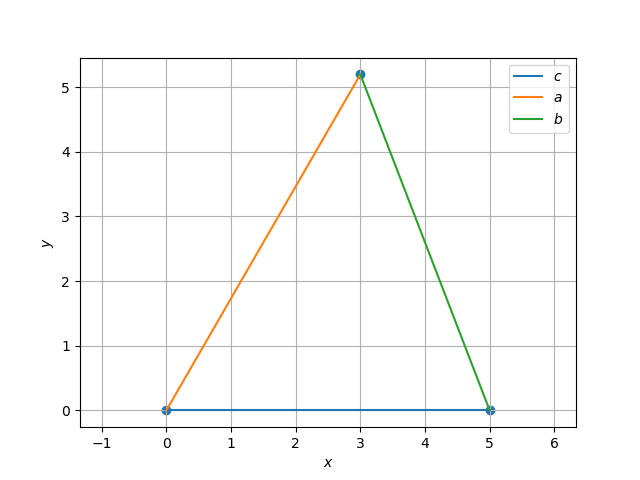
\includegraphics[scale=0.5]{plot}
    \caption{}
    \label{fig:plot}
\end{figure}
\end{document}
